\chapter{Initial Prototypes}

\section{Introduction}
Prototyping is an important part of any software engineering project,
as it enables the development team to demonstrate their progress to
their client in a way that they can more easily understand, and also
enables the client to clarify what they want from the system
\cite{brooks87}, \cite{sommerville11}.

In this chapter we describe the prototypes which have been used to
demonstrate EduCraft in its early development, along with how they were
received by those we showed them to. We first describe the mod which
was used in these demonstrations, and then explain the demonstrations
themselves.

\section{The `Dummy Mod'}
Both prototypes involved using something we called the `Dummy Mod'.
This was a simple mod which contained some basic custom items
which we believed would serve to demonstrate the goals which we were
aiming towards. Neither of the prototypes actually included any
elements that would be used in the finished product; rather, they served
simply to \textit{illustrate} what we hoped to achieve.

The premise of Dummy Mod was simple: we provided the player with a
customised weapon item (a `Dummy Sword'), and the means to generate a
number of modified enemies (`Dummy Zombies'). When a Dummy Zombie was
slain with a Dummy Sword, instead of dropping its usual items, instead it 
dropped a `Dummy Coin'. We also gave the means to combine nine of these coins 
into a `Pile of Dummy Coins', and to split a pile of coins into nine indvidual 
coins.

These basic implementations demonstrate what we hope to achieve in the
finished product, but with much less work: the code used to create the
items was minimal, pre-existing textures from within the game were
used instead of custom-made ones, and no special mathematical concepts
were implemented. The purpose was simply to illustrate that we could,
in principle, make a Minecraft mod which allowed players to use special
tools to collect particular items from enemies, which could then be
combined together.

\section{Demonstration to supervisor}
The first demonstration was carried out in a formal meeting with our
supervisor. This demonstration was very basic: we did not intent to present
anything approaching a working `level' of the game, but simply wished
to demonstrate that we knew how to work with Minecraft to produce mods.

In the demonstration, we gave the player a Dummy Sword, the means to spawn
(generate) a Dummy Zombie, and a crafting bench in order to combine the
coins into piles. The objective was very simple: the player spawned and
killed as many zombies as they wished, and made and destroyed piles of
coins as they wished.

\subsection{Feedback}
Feedback on this prototype was positive: it was clear from what was shown
that we knew what we were doing, and were able to produce mods that could
be used in a teaching environment.

The main criticisms of the prototype were visual. In an unmodified game of
Minecraft, zombies and other `undead' enemies burn in sunlight, and so for
the pursposes of the demonstration the game's time was set to night. Whilst
this is perfectly acceptable to an experienced Minecraft player, it was
suggested that to someone who had never played the game before, the darkness
might make it harder to understand what was going on.

It was also suggested that the perceived violence of the game might make it
harder to `sell' to schools---although the violence was fantasy, our
supervisor observed that the game still involved killing monsters with
swords. It was recommended that the game's graphics be modified to make
the mathematical focus more obvious.

\section{Demonstration at Southwold Primary School}
The second demonstration was much more involved, and was given to the
maths co-ordinator of Southwold Primary School, who would be responsible
for deciding whether or not to allow us to test our finished product
with children later on in the project. For this second demonstration, the
feedback received from the first prototype was incorporated and built upon.

Elements of the prototype are shown in Figure \ref{fig:prototype}.

\begin{figure}
\caption{Elements of the prototype level, clockwise from top left:
            1. the outer door, 2. the exit door and coin repository,
            3. the means of spawning zombies, 4. the created zombie}
\label{fig:prototype}
\centering
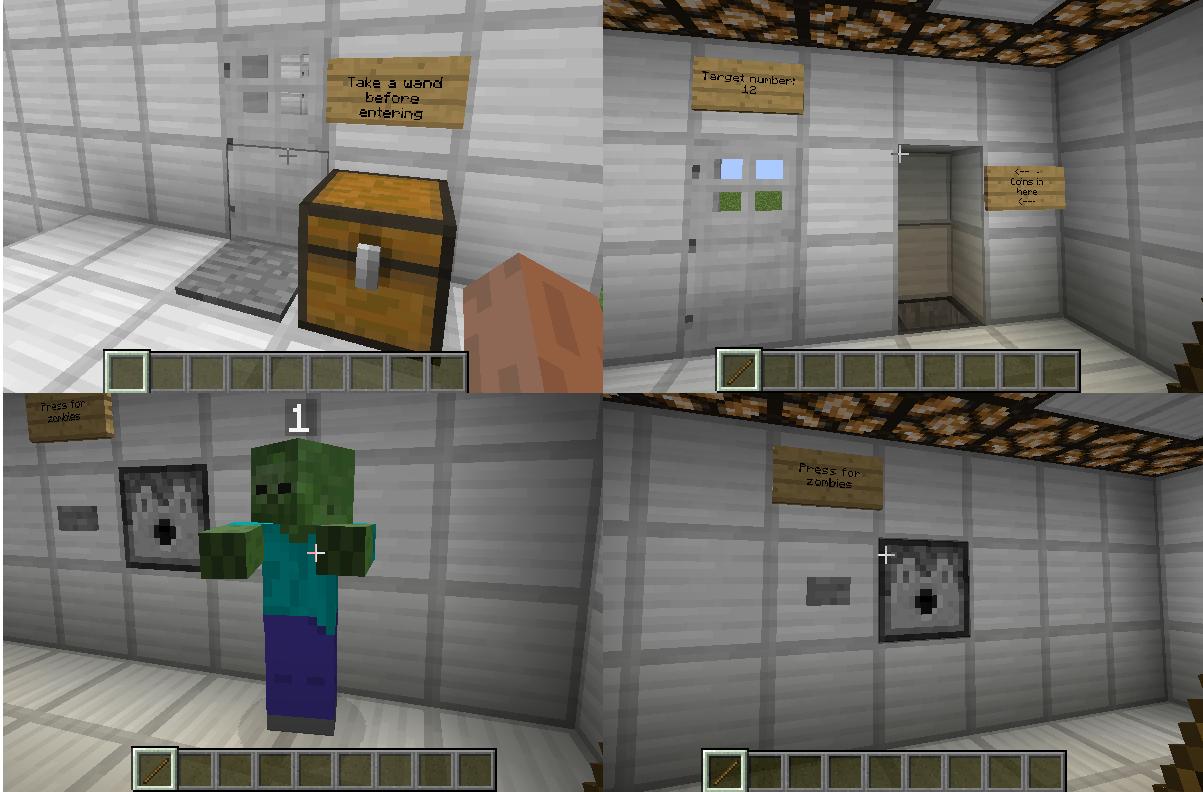
\includegraphics[width=13.5cm]{prototype-ssot-composite}
\end{figure}

\subsection{Level design}
For this demonstration, we created a simple level which used counting
as its main objective. The player's goal was to collect twelve
dummy coins and deposit them in a hopper; once the player had collected
and deposited twelve coins in this way, the door at the far end of the level
would open, allowing the player to progress.

The level was designed to be as minimalistic as possible, so as to 
demonstrate the possibility of creating mathematical puzzles in Minecraft
without distracting the teacher with other details of Minecraft gameplay.
The level conveyed the idea that we could build areas which players could not 
leave without first completing some problem---in this case, counting.

\subsection{Item design}
We decided that we could retain zombies in the game, as fighting monsters
formed an integral part of playing Minecraft which anyone who had seen the
game before would expect. Habgood's PhD work had already established that
it is acceptable for this sort of fantasy violence to be depicted in
educational games \cite{habgood07}, and so we felt that there was no
problem in retaining it.

We did redesign the player's `weapon', however---its texture was changed,
so that instead of appearing as a sword it was a simple stick, and it was
also called a `Maths Wand' instead of a Dummy Sword. We hoped this would
more clearly convey the mathematical nature of the game.

\subsection{Feedback}
The feedback for this second prototype was overwhelmingly positive. Despite
the teacher's complete lack of familiarity with Minecraft, she appeared
very excited by the prospect of being able to use it in lessons. She said
that she believed the level of violence would be acceptable, provided that
the emphasis was very clearly on the maths and not on the killing. This agreed
with what we had already heard from our supervisor.

Demonstrating the prototype also provided us with an opportunity to refine
our requirements, so that we could better direct our future work.
